%%%%%%%%%%%%%%%%%%%%%%%%%%%%%%%%%%%%%%%%%%%%%%%%%%%%%%%%%%%%%%%%%%%%%%%%%%%%%%%%
%2345678901234567890123456789012345678901234567890123456789012345678901234567890
%        1         2         3         4         5         6         7         8

\documentclass[letterpaper, 10 pt, conference]{ieeeconf}  % Comment this line out if you need a4paper

\IEEEoverridecommandlockouts                              % This command is only needed if 
                                                          % you want to use the \thanks command

\overrideIEEEmargins                                      % Needed to meet printer requirements.

\usepackage[bookmarks=true]{hyperref}
\usepackage{amsmath,algorithm}
\usepackage{amsfonts}
\usepackage[noend]{algpseudocode}
\usepackage{xcolor}
\usepackage{graphicx}
\usepackage{makecell}
\usepackage{float}
\usepackage{tikz}
\usetikzlibrary{positioning,shapes.misc}
\tikzset{
    myboxrectangle/.style={rectangle,draw=black,align=center, minimum width=2cm, minimum height=0.8cm},
}
\DeclareMathOperator*{\argmax}{argmax} % thin space, limits underneath in displays
\DeclareMathOperator*{\argmin}{argmin} % thin space, limits underneath in displays

\title{\LARGE \bf
Path-Tree planning using Rapidly-exploring Random Graphs for partially observable environments
}

\author{Camille Phiquepal$^{1}$, Andreas Orthey$^{2}$, Nicolas Viennot and Marc Toussaint$^{3}$
\thanks{$^{1}$Machine Learning \& Robotic Lab, University of Stuttgart, Germany
        {\tt\small camille.phiquepal@ipvs.uni-stuttgart.de}}
\thanks{$^{2}$Real time robotics, Berlin, Germany
        {\tt\small aorthey@rtr.ai}}
\thanks{$^{3}$Learning and Intelligent Systems Lab, TU Berlin, Germany
        {\tt\small toussaint@tu-berlin.de}}
}

\begin{document}



\maketitle
\thispagestyle{empty}
\pagestyle{empty}


%%%%%%%%%%%%%%%%%%%%%%%%%%%%%%%%%%%%%%%%%%%%%%%%%%%%%%%%%%%%%%%%%%%%%%%%%%%%%%%%
\begin{abstract}
This paper presents a new approach to path-planning for problems where essential and discrete aspects of the environment are partially observable.
To achieve its task, the robot must be able to observe and infer knowledge about its environement.
We introduce the ROPT (Random Optimal Path-Tree) algorithm which consists in planning a \textit{path-tree} in belief-space. Path-trees are tree-like motions with branching points where the robot receives an observation leading to a belief state update. The robot takes different branches depending on the observation received.
The algorithm has three main steps. First, a rapidly-exploring random graph (RRG) is grown. The RRG is grown similarly to RRT methods but has a graph structure. Second, the RRG is expanded to belief space by querying the observation model. In a third step, dynamic programing is performed on the belief space graph to extract a path-tree. The resulting path-tree combines exploration with exploitation i.e.\ it balances the need for gaining knowledge about the environment with the need for reaching the goal. We demonstrate the capabilities of the approach on navigation and mobile manipulation tasks.
% domain agnostic way
% More optimized towards likely states than unlikely ones
% modular algorithm
% exhibits exploration
% The planning procedure uses an observation model, inference
% generalizes rrt
% belief state
% inference
% react to observation
% in simulation on 2 kinds of examples (mobile robot, robot arm mounted on a robot arm)
\end{abstract}


%%%%%%%%%%%%%%%%%%%%%%%%%%%%%%%%%%%%%%%%%%%%%%%%%%%%%%%%%%%%%%%%%%%%%%%%%%%%%%%%
\section{INTRODUCTION}
In the field of path-planning, the environment is often assumed to be fully known. Partial observability, when considered, is often modelled as a limited and continuous variation around a central hypothesis  (e.g. addition of potential fields around obstacles, description of the robot localization uncertainty with gaussians). Planning itself is achieved using one single world representation.

In contrast, our approach aims to plan motions for problems where the robot knowledge about its environment is \textit{multi-modal}: The robot has a countable number of hypotheses about its environment. In practice, this can model obstructions in the environment the (see section \ref{experiement:navigation}), or the uncertainty about an object location (see section \ref{experiement:mobile_manipulation}), or any other uncertainty well represented as a discrete set of hypotheses.

This paper extends previous research work \cite{tamp-1}\cite{control-tree-1} which develop optimization based-methods for trajectory-tree planning in the respective subfields of Task and Motion Planning (TAMP) and Model Predictive Control (MPC). It extends the concept of tree-like motions to sampling-based path planning, and leverages the strengths of sampling-based approaches (especially the strong guarantees regarding collision avoidance and the asymptotic completeness) to tackle problems where the high number of occluding obstacles would be challenging for pure optimization-based methods (e.g. due to a high number of local minima). %environement complexity, environement structure, instead of occluding obstacles?
In addition, unlike \cite{tamp-1}, in which the observation actions are planned at the task level, the presented approach incorporates the observation model and the belief-state inference on the motion planning level directly, leading to unified algorithm.
% better sell the contributions?
%The main contribution of this work is

%The method is applicable to XXX and it is demonstrated on YYY

%This paper focuses on sampling based path planning. The main motivation for a sampling based methods in this context is the correlation between the observability problem and the collision avoidance problem, where sampling-based algorithm perform well: Partial observability is often due to obstacles occluding the robots field of view. In a similar way, obstacles prevent the robot to move freely. The ambition of the algorithm is to be a planning step solving both the problem of "where to move" and "where to observe" in complex environements.

%discrete partial observability vs continuous one -> DONE
%genesis
%motivation: strong link between observability pb and collision avoidance
%assumptions: multimodal - enumerable set of possible worlds, possibility to do inference
%integration in TAMP pipelines
%contribution / originality of the method: 
\section{RELATED WORK}
%A rich body of work has focused..

Path planning under partial observability and multi-modality of the environment state is related to the broader topic of path-planning under uncertainty for which many adaptations of classical sampling-based path planning algorithms like RRT \cite{lavalle1998rapidly} and PRM \cite{kavraki1996probabilistic} have been developed.

% use case: localization
One group such algorithms aims to tacke the localization uncertainty by planning paths which not only reach a goal but also minimize the localization uncertainty \cite{prentice2010belief} \cite{bry2011rapidly}. Like the presented approach, those algorithms plan in belief space on a grah grown in a sampling-based fashion. An observation model is used to infer the belief state dynamic. However, unlike the presented approach, those research model partial-observability over continuous variables (the localization), and assume gaussian belief-states. In addition we plan reactive path-trees reacting to the different possible observations.

% use case: mapping
Another closely related line of work plans paths maximizing the information gathered along the path \cite{hollinger2014sampling} \cite{levine2010information} \cite{dang2020graph}. Like the previously mentioned work, a graph or tree is grown in a sampling-based fashion. However, instead of planning in belief space, those approches determine the optimal traversal w.r.t. an information objective, e.g. volumetric gain for the use case of mapping in \cite{dang2020graph}.


% One line of work can be qualified as "observation-aware" algorithms where an observation model is used to
%The modeled uncertainty is typically the localization (either of the robot or of the obstacles). 
% use case: monitoring
Another direction of research uses sampling based methods for planning problems where the goal is expressed as a temporal logic specification \cite{karaman2009sampling} \cite{leahy2019control} \cite{vasile2020reactive}. Like the method of this paper, the ouput solution of the planning problem is more general than a sequence of states. In \cite{karaman2009sampling} \cite{vasile2020reactive}, the solutions are cyclic infinite paths. The closest to our proposed approach is \cite{leahy2019control}. It synthetizes control policies in belief space that react to observations. The goal is specified using GDTL (Gaussian Distribution Temporal Logic). Like the other belief space planning approaches previously mentionned (\cite{prentice2010belief} \cite{bry2011rapidly}), the considered uncertainty is over the robot localization, and belief states are modeled as gaussians. Kalman filters are used for the belief states update. In contrast, the presented approach focuses on the environment uncertainty, it doesn't assume gaussian beliefs but describes the environment uncertainty as a finite and countable set of hypotheses.
% extension of the GDTL
% transition system in belief space
% localization 
% feedback controller
% 2 stages
% synthetize control policy
% goal condition specifies constraints about the localization uncertainty
% uncertainty seen as noise
% FIRM Feedback Information Roadmap
% policy that satisfies the goal with a high enough satisfaction probability
% with the crucial difference that the uncertainty is continuous and over the robot localization and assumed to be gaussian. On the other hand our 
% belief update with kalman filter

%It  but can take the form of cycles.
%%XX is the closest related work

% connect to use case.. monitoring


%In particular xy show similaities with our approach in that the combine a first step of graph growing in belief space and second step of path extraction.

%Like our approach 

%path planning in the presence of goal uncertainty; 
%Belief space path planning
%Non-linear policies RRG
%View planning
%POMDP Navigation

\section{PROBLEM FORMULATION}

\begin{figure}[!htb]
 \center{\includegraphics[width=0.25\textwidth]{drawings/problem.pdf}}
 \caption{Example of planning problem: The robot must reach the goal area. The state of a door (open vs. closed) is only observable in its vicinity. }
 \label{fig:problem}
\end{figure}

\subsection{State representation}
The presented approach optimizes policies in a context of mixed-observability. The robot state is fully observable. On the other hand, discrete and essential parts of the environment are only partially observed. In the example of the Figure \ref{fig:problem} this models the fact that each door can be open or closed.
 
We consider a compound state representation where a state is composed of 2 parts:
\begin{itemize}
\item $x \in \mathbb{R}^n$ : is a continuous state and corresponds to the usual notion of state in the path planning litterature.
\item $s \in \mathcal{H}$ is a discrete state from a finite set of world hypotheses $\mathcal{H}$.
\end{itemize}

In the problem introduced on Figure \ref{fig:problem} the variable $s$ can take four possible values corresponding to the possible states of the environment as illustrated on Figure \ref{fig:multiple_worlds}.

\begin{figure}[!htb]
 \center{\includegraphics[width=0.45\textwidth]{drawings/multiple_worlds.pdf}}
 \caption{Partially observable discrete state: With 2 partially observable doors, there are 4 possible states of the environment.}
 \label{fig:multiple_worlds}
\end{figure}

Planning is performed is belief space, a belief state $b$ is a probability distribution over the different possible state hypotheses.

\subsection{Observation model}
\label{sec:observation_model}
The robot is not oblivious about the likelihood of each state hypothesis. For example, for the problem introduced on Figure \ref{fig:problem}, when the robot is in the vicinity of a door (symbolized with the circles), it receives an observation indicating whether the door is open or not. When an observation $o \in O$ is received, the belief state $b$ is updated according to a baysian update:
\begin{equation}
\label{eq:baysian}
b^\prime(s) = p(s | o) \times b(s), \forall s \in \mathcal{H},
\end{equation}
where $p(s | o)$ is the probability of being in state $s$ after receiving the observation $o$. 

In addition, we assume the observation model to be binary, meaning that $p(s | o) \in \{0.0, 1.0\}, \forall s \in \mathcal{H}, \forall o \in O$. This property is important. It guarantees that the number of belief-states is finite and can be ennumerated, which is needed for the graph expansion to belief state presented in Section \ref{section:graph_expansion_belief_space}. For the example of Figure \ref{fig:problem}, it means that observations indicate whether the door is open or not without uncertainty.

\subsection{Path-tree}
The algorithm consists in planning path-trees. As schematically shown on Figure \ref{fig:path_tree}, the path-tree starts from a single root node and finishes with leaf nodes satisfying the goal condition. The path-tree branches where the robot receives an observation leading to a belief state update. The different branches of the path-tree represent the different planned contingencies. To be complete, a path-tree must have a path going to the goal region for all $s \in \mathcal{H}$.

A consequence of the binarity of the observation model (see Section \ref{sec:observation_model}) is that the number of branchings $N_o$ stays small compared to the total number of states $N$ on the path-tree. In other words $N_o \ll N$. It can be understood easily on the presented example: once an observation has been received for a door, the agent knows with certainty if the door is open or not, such that the next observations of the same door don't lead to an update of the belief-state.

\begin{figure}[!htb]
 \center{\includegraphics[width=0.25\textwidth]{drawings/path_tree_example.pdf}}
 \caption{Example of path-tree: The path-tree branches where an observation leads to a belief state update. There are 2 planned contingencies for each branching corresponding to the 2 cases (door open or closed).}
 \label{fig:path_tree}
\end{figure}

We note a path-tree $\psi$. Nodes are composed of:
\begin{itemize}
\item a robot configuration $x$.
\item a belief state $b$ which corresponds to the knowledge of the robot regarding the discrete state $s$.
\end{itemize}

Edges are composed of:
\begin{itemize}
\item the observation $o$ which connects the belief states edge's incoming and outcoming nodes according to the update rule \ref{eq:baysian}.
\end{itemize}

In addition, we introduce the following notations:
\begin{itemize}
\item $\mathcal{L}(\psi)$ is the set of leaf nodes of the path-tree.
\item $b_u$ and $x_u$ refer respectively to the belief state and configuration of a node $u$.
\item $\forall (u, o, v) \in \psi$ ennumerates of the edges of the path-tree. It refers to the incoming node $u$, the outcoming node $v$ and the observation $o$ associated with the edge. 
\end{itemize}

\subsection{State validity}
We note $\mathcal{V}: S \times \mathbb{R}^n \rightarrow \mathbb{B}$ the function indicating if a state is valid (e.g. collision free). In general, the validity of a state depends on $s$. For example, on Figure \ref{fig:problem}, the states close to the door can be valid if the door is open but in collision if it is closed.
By extension, the validity predicate can be applied to a node $u$, a node is valid if the robot configuration $x$ is valid for all states having a non-zero likelihood,
\begin{equation}
\mathcal{V}(u) \iff \mathcal{V}(s, x_u), \forall s \in \mathcal{H}\ |\ b_u(s) > 0.
\end{equation}
% validity function provided from outside?

\subsection{State transitions validity and cost}
A transition between two nodes is valid if it corresponds to a valid, collision-free motion. Local planning between two configurations is not part of the planning algorithm is provided by the application layer and queried to validate sampled configurations. A valid transition between a pair of nodes $u, v$ is noted by the predicate $\mathcal{V}(u, v)$. 

In addition, a transition is associated with a cost $C(u, v)$ which indicates the motion cost from one tree node to another.

\subsection{Goal condition}
The goal condition is noted $G: S \times \mathbb{R}^n \rightarrow \mathbb{B}$. It is a function of both the partially observable discrete state $s$ and of the robot configuration. Having the condition depending on the discrete state can be usefull for use-cases where the robot searches for an object like in the experiment of Section \ref{experiement:mobile_manipulation}.
By extension, the goal predicate can be applied to a node $u$, a node is terminal if its configuration $x$ is terminal for all the states $s$ that have a likelihood greater than 0,
\begin{equation}
G(u) \iff G(s, x_u), \forall s \in \mathcal{H}\ |\ b_u(s) > 0.
\end{equation}
 
\subsection{Optimization Objective}
% plan for each contingency

The algorithm seeks to minimize the expected costs to goal. The probability to reach a node $v$ of $\psi$ can be derived from the initial belief state $b_0$ and the observation model, and we note this likelihood $p(v | \psi, b_0)$. 
The optimal path-tree $\psi^*$ is defined by:
\begin{subequations}
\label{eq:optimization_objective}
\begin{align}
\psi^* = &\argmin_{\psi} \sum_{(u, v) \in \psi} C(u, v) p(v | \psi, b_0), \label{eq:cost_min}\\
&\text{s.t.} \notag \\
&\forall s \in \mathcal{H}\ \exists\ l \in \mathcal{L}(\psi) \ |\ G(l), \label{eq:goal_constraint}\\
&\mathcal{V}(u, v), \ \forall (u, v) \in \psi \label{eq:validity}, \\
&b_v(s) = p(s | o) \times b_u(s), \forall s \in \mathcal{H}, \forall (u, o, v) \in \psi. \label{eq:belief_dynamic}
\end{align}
\end{subequations}

Equation \ref{eq:cost_min} is the minimization of the expected cost. \ref{eq:goal_constraint} is the constraint stating that the path-tree should be complete i.e. it should have a leaf satisfying the goal conditions for each possible $s$. \ref{eq:validity} specifies that each edge of the tree has to be a valid motion. Finally, \ref{eq:belief_dynamic} specifies the baysian update of the belief states along the tree (see \ref{sec:observation_model}).

It is noteworthy, that the problem formulation doesn't contain any term explicitely inciting the robot to explore its environment. The balance exploration / exploitation emerges naturally as a result of the minimization of the expected motion costs.
% difference compared to general POMDP
\section{Random Optimal Path-Tree algorithm (ROPT)}

\subsection{Overview}

To build a path-tree satisfying the specification of Equation \ref{eq:optimization_objective}, we proceed stepwise. First a transition system is grown in a sampling based fashion until the existence of a solution is guaranteed. This corresponds to the two first steps schematized on Figure \ref{algorithm_overview}. In a second step, the optimal path-tree is extracted using dynamic programming. 

\begin{figure}[!htb]
\scriptsize
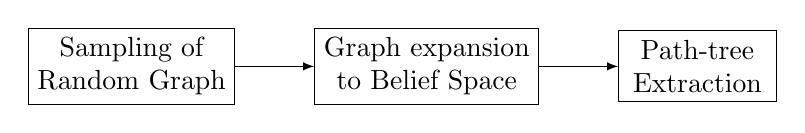
\begin{tikzpicture}[>=latex] 
\node[myboxrectangle] (RRG) {Sampling of\\ Random Graph};
\node[myboxrectangle] (BS) [right =of RRG] {Graph expansion \\to Belief Space} edge [<-] (RRG);
\node[myboxrectangle] (PO) [right =of BS] {Path-tree\\Extraction} edge [<-] (BS);
\end{tikzpicture}
 \caption{ROPT Algorithm overview. It contains three main steps corresponding to the algorithms described in the sections \ref{section:rapidly-exploring-random-graph}, \ref{section:rapidly-exploring-random-graph} and \ref{section:policy-extraction}.}
 \label{algorithm_overview}
\end{figure}

\subsection{Interface between the algorithm and the appication layer}

The connection between the core of the algorithm and a given planning problem is achieved via 4 functions that the application layer provides: 
\begin{itemize}
\item \textsc{StateCheck}, which takes a robot configuration $x$ as input and returns the list of worlds in which the configuration is valid.
\item \textsc{TransitionCheck}, which takes two robot configurations as inputs and returns the list of worlds in which the robot configurations is valid.
\item \textsc{GoalCheck}, which takes a robot configuration as input and returns the list of worlds in which the robot configuration fulfills the goal conditions.
\item \textsc{Observe}, which receives a robot configuration and a belief-state as inputs and returns the possible output belief states. %TODO: explain more% 
\end{itemize}

The functions \textsc{StateCheck}, \textsc{TransitionCheck} and \textsc{GoalCheck} are akin to the functions required by the RRT and PRM algorithms, but they are more general: the return type is a list of worlds instead of a boolean.

The \textsc{Observe} function is directly linked to partial observability and is specific to this algorithm. It allows belief-state inference. Going back to the example of Figure \ref{fig:problem}, \textsc{Observe} returns an unchanged belief-state for all robot configurations that are outside of the door visibility zone, this is because no observation can be received, and therefore no belief state inference is done. On the other hand, up to two possible belief-states are returned for robot configurations inside the door visibility zone. These two belief states correspond to the updated belief-states (see Section \ref{sec:observation_model}) for the two possible observations.
%It must be noted that the observations are not explicitely handled by the algorithm

The following sections detail how the calls to those functions are orchestrated by the algorithm to build a path-tree.

\subsection{Rapidly-exploring Random Graph}
\label{section:rapidly-exploring-random-graph}

In this first step, a random-graph is grown in a sampling based fashion. To avoid the curse of dimensionality, sampling is not performed in belief-space directly but in the robot configuration space. The random graph is an intermediate representation and will be expanded to belief-state in a second step as described in the next section.

The nodes of the random graph are associated with:
\begin{itemize}
\item a robot configuration $x$, which is randomly sampled.
\item a list worlds $\mathcal{F}$ in which the robot configuration is fulfilling the goal condition. This is obtained by querying the function \textsc{GoalCheck}. 
\end{itemize} 

The edges of the random graph are associated with:
\begin{itemize}
\item a list of worlds $\mathcal{W}$ in which the transition is valid. This is obtained by calling the function \textsc{TransitionCheck}.
\end{itemize}

%robot configurations are sampled (state $x$), then the environment model is queried to know in which worlds this state is valid. For example. The nodes of the random graph are 

% Sampling takes place in the state-space: the continuous robot configuration $x$ and the discrete state $s$ are sampled. Although planning will ultimately be performed in belief-space, the sampling at this stage is done in the state-space to avoid the curse of dimensionality. The random graph will be expanded to belief-state in a second step (see Section \ref{section:graph_expansion_belief_space}).

The random-graph creation is described in Algorithm \ref{alg:rrg}. First, the state is sampled (lines 4). Then the new state is steered from a neighbor node of the graph (line 7). Unlike RRT where the new state is state is steered from the nearest neighbor, here, the selected neigbhor is the nearest neighbor having world validities $\mathcal{W}$ containind the sampled world $w$ (line 5), as illustrated on Figure \ref{fig:expansion}. This additional condition for the neighbor selection is to ensure that the random graph contains paths to the goal for each world.
% similar to RRT / RRG quote RRG. The graph creation is done 
 
%The challenge is to efficiently grow a graph until completeness, i.e.\ up to a point guaranteeing that the next steps of the algorithm will be sucessfull (belief graph creation, path-tree extraction).

%unlike related work sample can be valid for certain worlds but not for others
%build transition system
%connect denser collision?free edges from this newly added vertex to its neighboring vertices within a defined radius ? .
% an off-line sampling-based algorithm for the construction of a global transition system

\begin{figure}[!htb]
 \center{\includegraphics[width=0.3\textwidth]{drawings/expansion.pdf}}
 \caption{Random Graph expansion: For a new sample \textit{a)}, the new state is computed steering from the closest compatible node of the graph. The closest compatible node depends on the sample world \textit{w}, see \textit{a)} and \textit{c}).}
 \label{fig:expansion}
\end{figure}
If the new state is valid for at least one world (line 9), the goal conditions are checked (line 10) and a new node is added to the random-graph (line 11).

Finally, the new node is connected to neighboring nodes (lines 13 to 16). The neighboring nodes are nodes within a given radius and which have world validities containing $w$.

This procedure is repeated until the graph is complete meaning that it will allow the sucessful extraction of a solution path-tree (see line 3). To implement the function \textsc{IsComplete} we assume in our examples that the transitions are \text-it{symmetrical}, i.e. if a motion exists from a node $u$ to $v$, then a motion between $v$ and $u$ also exists. Under this assumption, the random-graph contains a solution path-tree as soon as the set of leaf nodes is complete, in the sense that it covers every possible world, i.e.  $\bigcup_{u \in \mathcal{\mathcal{L}(G)}} \mathcal{F}_u = \mathcal{H}$. Indeed, the fact that the set of leaf nodes is complete implies that for each possible world $\forall s \in \mathcal{H}$, a path from the root to a leaf exists. An example of solution is therefore to execute those paths in sequence, and  potentially \textit{backtrack} to the root node if a path doesn't reach the goal (hence the required assumption regarding the symmetrical transition). In practice, once the completeness threshold is reached, a solution can be extracted which is typically way more optimal than the aforementioned worst-case backtracking strategy. In pratice we also typically introduce a minimum number of iterations, to make sure that the random-graph is expanded even beyond the completeness threshold to improve the quality of the path-trees. The assumption of symmetric transitions is fair for the examples considered in the experimental section, it could however be restrictive in the case of kinodynamic planning. %we inten in future work to... 

\begin{algorithm}[H]
\caption{Rapidly-exploring Random Graph}
\label{alg:rrg}
\begin{algorithmic}[1]
\Function{BuildRRG}{$q_{start}$}
	\State $\mathcal{G}$.\Call{init}{$q_{start}$}
	\While{$\neg$ \Call{IsComplete}{$\mathcal{G}$}  }
    	\State $q_{rand} \gets$ \Call{SampleState()}{}
    	\State $w \gets$ \Call{SampleWorld()}{}
    	\State $q_{near} \gets$ \Call{Nearest}{$q_{rand}, w$}
    	\State $q_{new} \gets$ \Call{Steer}{$q_{near}, q_{rand}$}
    	\State \textcolor{cyan}{\footnotesize/*get relevant info of the new state and add it to the graph*/}
    	\If{\Call{StateCheck}{$q_{new}$} $\neq \emptyset$}
    	    \State $\mathcal{F} \gets$ \Call{GoalCheck}{$q_{new}$}
    		\State $\mathcal{G}$.\Call{AddNode}{$q_{new}, \mathcal{F}$}
    		\State \textcolor{cyan}{\footnotesize/*get relevant edges info and add them to the graph*/}
    		\For{$q_{near} \in$ \Call{Nearests}{$q_{new}, w$}}
    			\State $\mathcal{W} \gets$ \Call{TransitionCheck}{$q_{near}, q_{new}$}
    			\If{$\mathcal{W} \neq \emptyset$}
    				\State $\mathcal{G}$.\Call{AddEdge}{$q_{near}, q_{new}, \mathcal{W}$}
    			\EndIf
    		\EndFor
    	\EndIf
    \EndWhile
\EndFunction
\Statex
\end{algorithmic}
\end{algorithm}

\subsection{Graph expansion to belief space}
\label{section:graph_expansion_belief_space}
%doesn't contain any geometric checks anymore, or calls to nearest-neighbors
%figure with several layers
At this stage, a random-graph $\mathcal{G}$ has been built, and the existence of a path-tree solution is guaranteed, however the random-graph is still intermediate representation that can't be used directly to optimize path-trees. In this step, a transition system in belief-space, or belief-graph $\mathcal{B}$ is constructed out of $\mathcal{G}$ and by querying the observation model. 
The nodes of the beief-graph are associated with:
\begin{itemize}
\item a robot-configuration $x$.
\item a belief-state $b$.
\end{itemize}
The edges of the belief-graph are associated with:
\begin{itemize}
\item the observation $o$ making the transition betwen the beliefs on the incoming and outcoming nodes.
\end{itemize}
The belief-graph can be understood as the random-graph replicated over several layers, where each layer is a different belief-state, as shown on Figure \ref{fig:belief_layers}. The transitions within on layer correspond to robot motions, whereas the transitions from one layer to another correspond to the integration of an observation leading to a belief-state update. The motion transitions are, in general, not identical across belief-states. For example, on Figure \ref{fig:belief_layers}, the transitions crossing through the doors exist only in beliefs compatible with an open door.
  
\begin{figure}[!htb]
 \center{\includegraphics[width=0.45\textwidth]{drawings/belief_graph.pdf}}
 \caption{Randon Graph expanded to belief state: The belief states are represented as \textit{layers} of the belief graph. The nodes within the observation range potentially lead to a belief state update and therefore have edges transitioning to other belief states (thick vertical edges).}
 \label{fig:belief_layers}
\end{figure}

The construction procedure is given by the Algorithm \ref{alg:belief}. First, the edges of $\mathcal{G}$ are replicated to the belief-states compatible with the edge's valid worlds (line 3 to 7).

Second, the observation model is called via the function \textsc{OBSERVE} to identify where edges should be created between belief-states (lines 9 to 12). The belief-state-transition edges due to observations are represented by vertical lines going from one layer to another on Figure \ref{fig:belief_layers}.

\begin{algorithm}[H]
\caption{Creation of the belief graph}
\label{alg:belief}
\begin{algorithmic}[1]
\Function{BuildBeliefGraph}{$b_{start}, \mathcal{G}$}
	\State \textcolor{cyan}{\footnotesize/*connect nodes within the same belief*/}
	\For{$e \in$ $\mathcal{G}.edges$}
		\For{$b \in$ \Call{Beliefs}{$e.world\_validities$}}
			\State $u \gets \mathcal{B}$.\Call{AddNode}{$b, e.from$}
			\State $v \gets \mathcal{B}$.\Call{AddNode}{$b, e.to$}
			\State $\mathcal{B}$.\Call{AddEdge}{$u, v$}
		\EndFor
	\EndFor
	\State \textcolor{cyan}{\footnotesize/*create transitions between beliefs due to observations*/}
	\For{$u \in$ $\mathcal{B}.nodes$}
	   	\State $V \gets$ \Call{Observe}{$u$}
		\For {$v \in V$}
			\State $\mathcal{B}$.\Call{AddEdge}{$u$, $v$}
		\EndFor
	\EndFor
\EndFunction
\end{algorithmic}
\end{algorithm}

%No need to query the collision checks anymore%
The belief-graph $\mathcal{B}$ is significantly larger than the random graph $\mathcal{G}$ due to the different belief-states corresponding to one same robot configuration. However, its construction only calls the observation model (function \textsc{Observe}). In contrast, the random-graph is smaller but its creation requires calls the collision checks (\textsc{StateCheck} and \textsc{TransitionCheck}) as well as the nearest neighbor search that are expensive.

\subsection{Policy extraction}
\label{section:policy-extraction}

At this stage, the belief-graph $\mathcal{B}$ is fully built, and it contains at least one path-tree satisfying the goal conditions (see \ref{eq:goal_constraint}). The goal is now to find the optimal path-tree by minimizing the expected costs to goal (see \ref{eq:cost_min}).

The expected costs to goal are computed for each node of $\mathcal{B}$. This is done using dynamic programming and by iteratively applying a Bellman updates on each node of $\mathcal{B}$.
The procedure is described by the Algorithm \ref{alg:expected_costs}.

The algorithm is similar to the Dijkstra algorithm \cite{Sniedovich2006DijkstrasAR} in the way the nodes are prioritized using a priority queue (lines 2 to 13). For edges corresponding to a robot motion, the Bellman update is also the same as in Dijkstra (lines 15 and 16). However, for edges corresponding to an observation, the Bellman update of the parent node differs and is the sum of the children expected costs weighted by their respective branching probabilities (lines 17 to 19).
\begin{algorithm}[H]
\caption{Computation of the expected costs to goal}
\label{alg:expected_costs}
\begin{algorithmic}[1]
\Function{ComputeExpectedCostToGoal}{$\mathcal{B}$}
	\State $Q \gets $ \Call{PriorityQueue()}{}
	\State \textcolor{cyan}{\footnotesize/*Initialization*/}
	\For{$n \in$ $\mathcal{B}.nodes$}
		\If{\Call{IsFinal}{$n$}}
			\State $C[n] \gets 0.0$
			\State $Q$.\Call{Push}{$n, 0.0$}
		\Else
			\State $C[n] \gets +\infty$
		\EndIf
	\EndFor
	\State \textcolor{cyan}{\footnotesize/*The main loop*/}
	\While{$\neg$ \Call{IsEmpty}{$Q$}}
		\State $v \gets$ \Call{Pop}{$Q$}
		\For {$u \in$ \Call{Parents}{$v$}}
			\State \textcolor{cyan}{\footnotesize/*Bellman update dependant on the edge type*/}
			\If{\Call{IsActionEdge}{$u, v$}}
				\State $c \gets$ \Call{Cost}{$u$}$+ C[v]$
			\ElsIf{\Call{IsObservationEdge}{$u, v$}}
				\State $\mathcal{W} \gets $ \Call{ObservationChildren}{$u$}
				\State $c \gets \sum_{\nu \in \mathcal{W}}{ p(\nu | u) \times C[w]} $
			\EndIf
			\If{$c < C[u]$}
				\State $C[u] \gets c$
				\State $Q$.\Call{Push}{$u, c$}
			\EndIf
		\EndFor
	\EndWhile
\EndFunction
\end{algorithmic}
\end{algorithm}

Once the expected costs to goal are known for ech node, the optimal path-tree can be built straighforwardly starting from the root and recursively appending the best next child, or next best children (in case of a node with an observation branching).

Optimizing w.r.t. the expected costs to goal naturally results in an exploration vs. exploitation trade-off, i.e. path-trees balance the need for moving towards configurations  providing informative observations vs. the need to advance towards the goal.
%balance exploration and exploitation

\subsection{Path-tree refinement}
%partial shortcut on trajectory pieces%
At this stage, a solution path-tree has already been extracted. However path-trees may contain  unnatural or jerky motions due to the random nature of the random-graph creation. One way to reduce this phenomenon is to have a high minimal number of iterations when creating the random-graph. However, this can become quite costy in terms of runtime. In practice, it is also very fast and efficient to improve the path-tree in a final refinment step. We refine the path-tree piecewise: the path-pieces between observation branchings are refined independently using the partial-shortcut method \cite{geraerts2007creating}. The branching nodes corresponding to observations are extremities of the path pieces and they form the junctions between path pieces. Those nodes are not modified by the refinement procedure. 

%Obtaining near-optimal observation points therfore relies on having  
%\subsection{Complexity analysis} -> keep for Phd
% rename to algoritmic properties (completness, optimality)

% (i.e., it finds a solution with probability 1 if one exists and the number of samples approaches infinity)

%w.r.t. the number of beliefs
% different problems lead to different relation n_world <-> n_beliefs

\section{EXPERIMENTS}
The path-planner core algorithm is implemented in the Rust programming language \cite{matsakis2014rust}. The application layer is implemented in C++ using MoveIt \cite{coleman2014reducing}. The source code and a supplementary video are available for reference \footnotemark \footnotetext{\href{https://github.com/cambyse/po-rrt}{https://github.com/cambyse/po-rrt}}. %TODO put real url

\subsection{Mobile robot navigation} \label{experiement:navigation}

\subsection{Robot arm object fetching} \label{experiement:mobile_manipulation}
In these two examples, the robot is composed of a Panda arm mounted on a mobile base. The robot task is to pick-up an object which location is unknow (see Figure \ref{fig:arm_example_1} and \ref{fig:arm_example_2}). The robot has prior knowledge of several potential locations, but the actual location is unknown at planning time. 

%. In other words, the perception pipeline will detect the object if the object is within the filed of view, at a distance closer than 2 meters from the sensor, and that the object is not occluded (e.g. by the walls).

%TODO: 
% - put tables to avoid the unused slots?
% - just oneblock?
% - picture sensor field of view etc?
\begin{figure}[!htb]
 \center{\includegraphics[width=0.45\textwidth]{drawings/2_arm/example_1.png}}
 \caption{Example 1: The robot has to pick the green block. The block location is unknown, it maybe on each one of the three shelves.}
 \label{fig:arm_example_1}
\end{figure}

The observation model simulates that a sensor is placed on the robot gripper and that the perception pipeline detects the block when it is within the sensor field of view (60$^{\circ}$), at a distance less 2 meters that from the sensor, and not occluded by other objects (e.g. the walls).

\begin{figure}[!htb]
 \center{\includegraphics[width=0.45\textwidth]{drawings/2_arm/example_2.png}}
 \caption{Example 2: The block might be on two different shelves. The opening between thw two doors potentially allows the robot to observe the shelves without entering the rooms.}
 \label{fig:arm_example_2}
\end{figure}

Planning is performed in joint space with 9 degrees of freedom (2 for the base, and 7 for the robot arm).

Figure XX shows the trajectory of the 

\begin{figure}[!htb]
 \center{\includegraphics[width=0.45\textwidth]{drawings/2_arm/example_1_path_tree.png}}
 \caption{Path-tree: The planned path tree first moves towards the shelf\_0 to reach the first viewpoint. If the object is on the shelf\_0, the green path is executed. Otherwise the robot moves towards the second viewpoint. Based on the observation, the robot executes either the magenta or the orange path.}
 \label{fig:example_1_path_tree}
\end{figure}

\begin{figure}[!htb]
 \center{\includegraphics[width=0.45\textwidth]{drawings/2_arm/example_2_viewpoint.png}}
 \caption{Observation branching point: A first common branch of the path-tree leads the robot to an observation point through the opening. Based on the received observation, the robot will either execute the yellow or the magent path.}
 \label{fig:example_2_view_point}
\end{figure}

%example of path tree, show the view-point

%table runtime, first 

%influence of the number of iterations on thequality

% influence of the belief state

% Observation model
% Runtime per algorithm stage

\begin{table}[h]
\begin{center}
\begin{tabular}{|c||c|c|c|c||c|}
\hline
  & \thead{\# of\\ iter} & \thead{random\\graph\\creation} & \thead{belief-\\space\\expansion} & \thead{policy\\ extraction} & \thead{planning\\time\\(ms)} \\
\hline
example-1  & & & & &\\
 & & & & &\\
\hline
example-2  & & & & &\\
 & & & & &\\
\hline
\end{tabular}
\end{center}
\caption{Planning times:.}
\label{tab:table_obstacle_avoidance}
\end{table}

% variation 3 locations vs 9 locations or tables?

\section{CONCLUSIONS AND FUTURE WORK}

%%%%%%%%%%%%%%%%%%%%%%%%%%%%%%%%%%%%%%%%%%%%%%%%%%%%%%%%%%%%%%%%%%%%%%%%%%%%%%%%



%%%%%%%%%%%%%%%%%%%%%%%%%%%%%%%%%%%%%%%%%%%%%%%%%%%%%%%%%%%%%%%%%%%%%%%%%%%%%%%%



%%%%%%%%%%%%%%%%%%%%%%%%%%%%%%%%%%%%%%%%%%%%%%%%%%%%%%%%%%%%%%%%%%%%%%%%%%%%%%%%
\section*{ACKNOWLEDGMENT}


%%%%%%%%%%%%%%%%%%%%%%%%%%%%%%%%%%%%%%%%%%%%%%%%%%%%%%%%%%%%%%%%%%%%%%%%%%%%%%%%

\bibliography{references}
\bibliographystyle{ieeetr}

\end{document}
